\section*{Del 2: Kostnadsestimering}

	\subsection*{Oppgave 1}
		{\bf Identifiser 5-6 årsaker som har medvirket til kostnadsoverskridelse
		i dette prosjektet. Hva ville du ha gjort annerledes dersom du var prosjektansvarlig?}

		{\bf Årsaker til kostnadsoverskridelse:}
		\begin{itemize}
			\item {\bf Årsak 1 - Feil fokus:} De tenkte mer på mulighetene for videresalg og 
			det å skaffe seg ny kunnskap i tillegg til at de ville bruke sin nye sharepointkonsulent 
			fordi de ikke hadde noe å gjøre på denne tiden.
			\item {\bf Årsak 2 - Dårlig prosjektvirksomhet:} De hadde ikke noen særlige rutiner når det 
			gjaldt prosjektledelse, noe som kom godt til syne da det ikke var lagt planer for hvordan 
			man skulle gjennomføre prosjektet. Samtidig er det litt ironisk at noen med lite erfaring
			innen prosjektstyring skal lage et verktøy for å håndtere den type arbeid. 
			\item {\bf Årsak 3 - Dårlig kommunikasjon med kunde:} De hadde ikke særlig kontakt med kunde og 
			visste ikke hvilke regler de måtte forholde seg til i forhold til sikkerhet og andre 
			infrastrukturelle forhold. I tillegg visste de heller ikke om kundens frist da kunden 
			ikke hadde sagt noe om denne.
			\item {\bf Årsak 4 - Endringer i krav:} Kravene gikk ut på hvordan de jobbet i dag og 
			ikke hvordan de hadde lyst til å jobbe framover. Dette førte til at kravene ikke 
			nødvendigvis stemte med det kunden ville ha.
			\item {\bf Årsak 5 - Opplæring av systemet:} De hadde ingen plan for å lære opp kunden i 
			hvordan systemet fungerte, noe som førte til at det ble vanskelig å sette av tid da 
			mange av brukerne var ute på andre prosjekter til ulike tider og deres hovedkontakt 
			var ute i fødselspermisjon. De måtte også som en konsekvens av dette bruke mye tid på å
			reise til kunden for oppsett på klientsiden. 
			\item {\bf Årsak 6 - Holdt ikke løfter:} De lovte mye mer enn det de visste de kunne holde. 
			De hadde ikke helt oversikt om kunnskapen som trengtes for å levere det de lovte.
			Dette førte til at underleverandør måtte ta over ferdigstilling av prosjekt med belønning fra
			kontraktsummen. 
		\end{itemize}

		\clearpage
		{\bf Hva ville vi forbedret om vi hadde ansvaret?}
		\begin{itemize}
			\item {\bf Kontrakter og avtaler:} som en av de største utgiftspostene var avtalene de gjor
			med underleverandøren. Når de selv ikke kunne levere måtte de ty til hjelp fra underleverandør
			som tok timepris, en variabel kostnad. Hvis jeg hadde ansvar for prosjektet vill jeg
			nok i utgangspunktet ikke tatt dette prosjektet når man må leie inn essesnsiell kunnskap fra
			en underleverandør, men om jeg måtte hadde jeg ikke inngått en avtale med variable kostnader og
			mangler i forhold til ferdigstilling. 1) Fast pris 2) underleverandør må hjelpe til med integrering
			av løsning.
			\item {\bf Kommunikasjon med kunde:} det virket ikke som om de har hatt noe form for kommunikasjon
			med kunde. Det er mangler på krav og kunnskap inn i bildet. Som prosjektansvarlig ville jeg
			startet et prosjekt med spørsmål som "når skal det ferdigstilles?". En grunn til dette er at jeg 
			ville gjennomført en god planlegging av prosjektet med tanke på timeplan og ressursbruk. Dette er vanskelig
			når slik informasjon ikke er planlagt. Ofte kan "skjult" informasjon få store konsekvenser om man
			ikke vet om det på forhånd. 
			\item {\bf Samle domenekunnskap:} det blir nevnt at bedriften ikke hadde noe spesiell tyngde innenfor
			prosjektstyring. Siden dette var et verktøy for prosjektsyring er det viktig å brukerene å bli godt kjent
			med dem for å vite hva de trenger å levere. Dette vil dekke noe av kunnskapsgapet. 
			\item {\bf Vudering av lønnsomhet:} dette virker som et skrekkeksempel på hvor man ikke skal ta 
			på set et slikt prosjekt. Som det nevnes i årsak 1 ble prosjektet tatt på feil grunnlag. Hvis de
			hadde tatt en mer grundig analyse av situasjon ville man kanskje unngått å satt seg i en økonomisk 
			dårlig situasjon som de nå klarte til slutt. 
			\item{\bf Vurdere egen kompetanse og ressurser:} Det virker ikke som om de satte spørsmål med sin egen
			kompetanse. Som ansvarlig ville jeg gjennomgått en analyse på kompetanse og ledige ressurser. 
			Hvis dette ikke er på plass kan man se en tydelig risiko med å ta et slikt prosjekt. 
			\item{\bf Organisering av opplæring:} for å ikke få kostnadene for opplæring må dette organiseres og 
			avtales på et tidlig tidspunkt. Dette krever at de har avtalt med kunden når systemet
			skal settes i produksjon. 
		\end{itemize}

	\clearpage
	\subsection*{Oppgave 2}
		{\bf Hvorfor er kostnadsestimering en så viktig komponent i prosjektplanlegging? Diskuter hvordan det
		linkes sammen med WBS og prosjektplan.}

		WBS: deler prosjektet opp i mindre deler
		Prosjektplan: strukturerer opp varighet, avhengigheter og ressursbruk

		Nå man skal gjøre kostnadsestimering må man i utgangspunktet vite hvilke deler av prosjektet man 
		skal estimere. Å estimere et stort prosjekt som en helhet kan være vanskelig fordi et prosjekt
		består av mindre deler. Ved å ha en klar oppdeling av prosjektet i mindre pakker er det lettere
		å gjøre en estimering av kostnad på de mindre delene.

		I en prosjktplan legges de små pakkene utover i en tidsplan med tanke på varighet, avhengigheter og
		ressurser. I en slik plan få man se tidsperspektivet og det er lettere å gi et klart bilde av hvordan
		prosjektets gang vil gå. Sett uten å lage en prosjektplan vil man naturlig bare summere opp alle aktiviteter
		som en sekvens av aktiviteter og dele dette opp på totalt antall ressurser. 
		Det man ofte må ta hensyn til er at noen aktiviteter avhenger av andre aktiviter, noe som gjør at noen aktiviteter
		som egentlig tar 5 uker ikke kan ferdigstilles før 7 fordi den må vente 2 uker på en annen aktivitet.
		Dette er viktig å ta hensyn til når man gjør kostnadsestimering fordi slike aktiviteter påvirker
		estimatene. 

		Gjør man en oppsummering av dette ser man at alle disse bitene har en klar kobling! 
		Samler man alle disse aktivitetene ser man at dette utgjør hovedområdene innen projektplanlegging. 
		Planlegge med tanke på: Aktiviteter (WBS), Tid (Prosjektplan), og kostand (Kostnadsestimering).

		Hvis man ikke gjør en grundig kostnadsestimering kan et prosjekt gå skikkelig å grøfta for
		både kunde og leverandør.

		\begin{figure}[H]
			\centering
			
\includegraphics[scale=0.2]{task3.png}
		\end{figure}

	\clearpage
	\subsection*{Oppgave 3}
		{\bf Oppgaveinformasjon:}
			\begin{table}[H]
			\begin{tabular}{ >{\centering\arraybackslash}p{1.5cm} | >{\centering\arraybackslash}p{1.7cm} | >{\centering\arraybackslash}p{2.35cm} |  >{\centering\arraybackslash}p{0.75cm} | >{\centering\arraybackslash}p{0.75cm} |
			>{\centering\arraybackslash}p{0.75cm} | >{\centering\arraybackslash}p{0.75cm} | >{\centering\arraybackslash}p{1cm} }
				{\bf Activity} & {\bf Duration} & {\bf Predecessors} & {\bf ES} & {\bf EF} & {\bf LS} & {\bf LF} & {\bf Slack} \\ \hline
				A & 3 & - & 0 & 3 & 0 & 3 & - \\ \hline
 				B & 5 & A & 3 & 8 & 8 & 13 & 5 \\ \hline 
				C & 7 & A & 3 & 10 & 3 & 10 & - \\ \hline
				D & 3 & B, C & 10 & 13 & 10 & 13 & - \\ \hline
				E & 5 & B & 8 & 12 & 13 & 17 & 5 \\ \hline
				F & 4 & D & 13 & 17 & 13 & 17 & - \\ \hline
				G & 2 & C & 10 & 12 & 15 & 17 & 5 \\ \hline
				H & 5 & E, F, G & 17 & 22 & 17 & 22 & - \\ \hline
			\end{tabular}
		\end{table}

		{\bf a) Konstruer nettverket ved bruk av AON notasjon}

			\begin{figure}[H]
				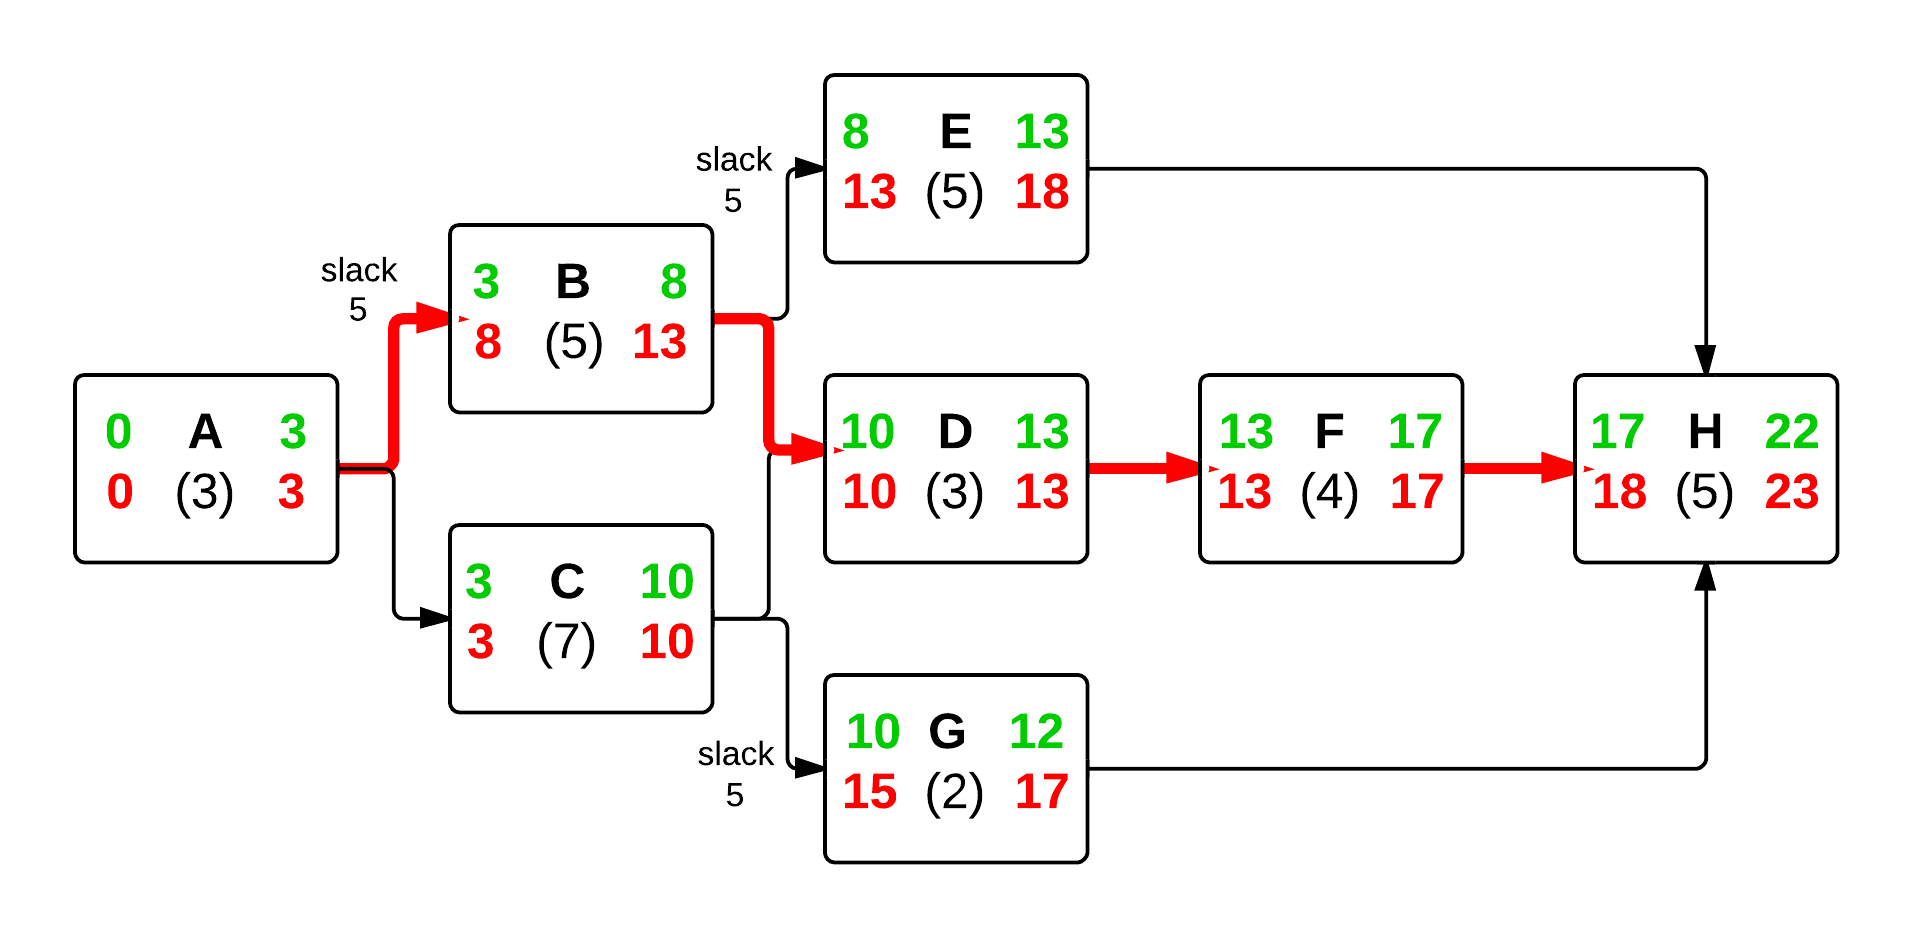
\includegraphics[width=\textwidth]{task7.png}
			\end{figure}

		{\bf b) Identifiser kritisk sti og alle mulige stier i nettverket}

			{\bf Kritisk sti:} A-B-D-F-H (vises i rødt i nettverket)
			{\bf Andre stier:}
			\begin{itemize}
				\item A-B-E-H
				\item A-B-D-F-H (kritisk)
				\item A-C-D-F-H
				\item A-C-G-H
			\end{itemize}


